\epstopdfsetup{outdir=./}
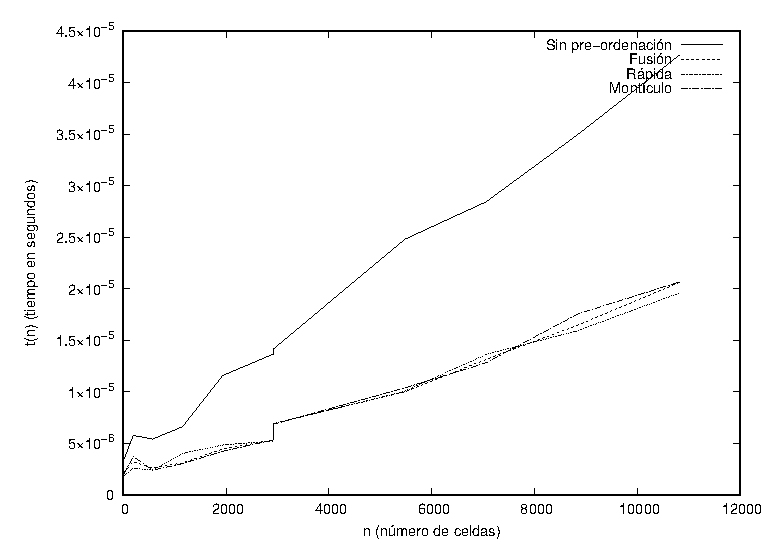
\includegraphics{graphic.eps}
\begin{lstlisting}
    
    
    placeDefenses3(bool** freeCells, int nCellsWidth, int nCellsHeight, float mapWidth, float mapHeight
    , List<Object*> obstacles, List<Defense*> defenses) {
        
        float cellWidth = mapWidth / nCellsWidth;
        float cellHeight = mapHeight / nCellsHeight; 
        cronometro cNoOrder, cQuickSort, cFusion, cHeap;
        int rNoOrder = 0, rFusion = 0, rQuickSort = 0, rMonticulo = 0; 
        
        for(int it = 0; it<4; it++){
            
            std::vector<std::vector<float>> MapValue(nCellsHeight, std::vector<float>(nCellsWidth));
            int maxAttemps = 1000;
            std::vector<cellValueStruct> cells;
            
            for(int i = 0; i < nCellsHeight; i++){
                for(int j = 0; j < nCellsWidth; j++){
                    MapValue[i][j] = defaultCellValue(i, j, nCellsWidth, nCellsHeight, mapWidth, mapHeight, obstacles, defenses);
                    }
                    }
                    
                    
                    for(int i = 0; i < nCellsHeight; i++){
                        for(int j = 0; j < nCellsWidth; j++){
                            cells.push_back(cellValueStruct(i, j, MapValue[i][j]));
                            }
                            }
                            
                            
                            switch(it){
                                case 0:
                                cNoOrder.activar();
                                sort(cells.begin(), cells.end(), compare());
                                
                                case 1: 
                                cFusion.activar();
                                sortFusion(cells, 0, cells.size()-1); 
                                
                                break;
                                case 2:   
                                cQuickSort.activar();
                                quickSort(cells, 0, cells.size()-1); 
                                
                                break;
                                case 3: 
                                cHeap.activar();
                                heap(cells); 
                                
                                break;
                                }
                                
                                
                                Vector3 v;
                                int i = cells.size()-1;
                                int row, col;
                                bool condition=true;
                                
                                for( List<Defense*>::iterator currentDefense = defenses.begin(); currentDefense != defenses.end() && maxAttemps > 0 && condition; maxAttemps--, i--){
                                    
                                    if(it!=0) v = cellCenterToPosition(cells[i].x, cells[i].y, cellWidth, cellHeight);
                                    else v = selection(cells, cellWidth, cellHeight);
                                    positionToCell(v, row, col, cellWidth, cellHeight);
                                    if(feasibility((*currentDefense)->id, row, col, nCellsWidth, nCellsHeight, mapWidth, mapHeight, obstacles, defenses)){
                                        maxAttemps = 1000;
                                        (*currentDefense)->position = v;
                                        cells.erase(cells.begin()+i);
                                        i=cells.size()-1;
                                        currentDefense++;
                                        } 
                                        
                                        
                                        switch(it){
                                            case 0 :
                                            rNoOrder++;
                                            condition = cNoOrder.tiempo() < (0.01 / (0.001 + 0.01));
                                            break;
                                            case 1: 
                                            rFusion++;
                                            condition = cFusion.tiempo() < (0.01 / (0.001 + 0.01));
                                            break;
                                            case 2:   
                                            rQuickSort++;
                                            condition = cQuickSort.tiempo() < (0.01 / (0.001 + 0.01));
                                            break;
                                            case 3: 
                                            rMonticulo++;
                                            condition = cHeap.tiempo() < (0.01 / (0.001 + 0.01));
                                            break;
                                            }
                                            
                                            }
                                            
                                            
                                            
                                            switch(it){
                                                case 0:
                                                cNoOrder.parar();
                                                case 1: 
                                                cFusion.parar();
                                                break;
                                                case 2:   
                                                cQuickSort.parar();
                                                break;
                                                case 3: 
                                                cHeap.parar();
                                                break;
                                                }
                                                
                                                if(it!=0) cells.clear();
                                                }
                                                
                                                std::cout << (nCellsWidth * nCellsHeight)
                                                << '\t' << cNoOrder.tiempo() / rNoOrder
                                                << '\t' << cFusion.tiempo() / rFusion
                                                << '\t' << cQuickSort.tiempo() / rQuickSort
                                                << '\t' << cHeap.tiempo() / rMonticulo
                                                << std::endl;
                                                }
\end{lstlisting}